\documentclass[pageno]{jpaper}
\usepackage{multicol}
\usepackage{graphicx}
\graphicspath{ {images/} }

\newcommand{\IWreport}{2017}
\newcommand{\quotes}[1]{``#1''}


\widowpenalty=9999

\usepackage[normalem]{ulem}
\begin{document}

\title{
The Feed:\\
A Decentralized Photo Sharing Application Built Using the Blockchain}

\author{Oluwapelumi Odimayo \\Partner: Michael Friedman Adviser: Michael J. Freedman}

\date{}
\maketitle
\fontsize{10.2}{1.2}\selectfont

\begin{multicols*}{2}
\thispagestyle{empty}


\begin{abstract}

Decentralized applications built on top of blockchains have garnered much attention in recent years for the security properties afforded to them by these peer-to-peer (P2P) networks. The rise in popularity of these applications can be attributed to growing security and privacy concerns associated with traditional web application models. However, this departure also led to a departure from a traditional user experience. Specifically, although these applications remove the role of a central “network overseer” that can see all user data going through the network, they hinder the ease of use and connectivity of traditional web applications. On top of this, those applications that use and incentivize their own blockchain incur costs on the user that could hinder access.\par
In this paper we introduce the design of The Feed, a decentralized photo-sharing application built using the Blockstack platform. The goal of this application is to give users control of their data and eliminate the role of the network overseer. Furthermore, users will be able to join and leave the network freely i.e. they can completely remove (access to) their data from the network. The Feed is an instagram-like social network that is easy for the end-user to setup and use. It eliminates the costly operations associated with other decentralized applications by reducing interaction to the blockchain by only using it as a login and authorization/verification services. The design presented is such that the security properties of the Blockstack platform are used to provide users with a network in which they own/control their data and, more importantly, no longer have to trust a central node or “network overseer” to participate in the network.  Users will be able to join and leave the network freely i.e. they can completely remove (access to) their data from the network. The Feed makes acceptable tradeoffs in performance for increased security and privacy.

\end{abstract}


\section{Introduction}

The advent of social networks like Twitter\footnote{https://twitter.com/}, Facebook\footnote{https://www.facebook.com/}, and Instagram\footnote{https://www.instagram.com/} have ushered in an era of unprecedented connectivity. Never before has it been so easy to connect and share with individuals from around the world. These applications provide a platform upon which the majority of online communication takes place today. With this, however, there are growing security and privacy concerns associated with these networks. A large contributing factor to these concerns is how the entities which control these networks (e.g. Facebook) use user data. On one hand, these websites collect user data to iteratively improve user experience for the entire network overall producing a general good the user base.\par 
For example, Facebook faced serious backlash when it was made public that the company had been running a research experiment on its user base to see if they could, without their knowledge, affect a user’s mood.(cite FB Paper) This incident brought to light two key aspects of the traditional social network model that user’s must consent to to participate in the network. This first being that the user must give up ownership of their data and the second is that the user must allow some central entity, in this case Facebook, to be able see and process all of their content.\par
Traditional social networking applications have the following general architecture:\newline

\begin{center}
	\begin{itemize}
		\setlength{\itemsep}{2\baselineskip}
		\item A client/user that wishes to access the network.\\
		\item A central node and point of trust through which all user’s communicate within the network and all on which all user data is stored.\\
		\item A network overseer that is able to view all information stored on the network and all communication that goes through the network.\newline
	\end{itemize}
\end{center}

Recently, these user focused concerns have brought about various “decentralized applications” designed to give users control over their data and to eliminate the centralize network overseer entity. A lot of these applications are built on top of blockchains which essentially provide a verified naming system, but, as a consequence, many operations on these networks require microtransactions to propagate them throughout the network. Furthermore, these applications dramatically change the user experience found in traditional social networking applications. Additionally, while these applications do remove control of a user’s data from the central node, they don’t give the user complete control. They cannot completely remove their trace from the network as that would require making changes to the underlying blockchains. The primary motivation for The Feed is to create a system architecture that solves these issues.\par
The goal for this project is to build a social network archicture in which users own their data and do not have to trust a central network overseer  to participate in the network. At any point a user should be able to completely remove any trace that they were on the network without changing how the rest of the network operates. Furthermore, the design of this application seeks to eliminate the “per operation” costs of other contemporary decentralized applications. Specifically, users will only need to purchase a .id namespace to gain access to the network. Once that is completed a user will not have to pay microtransactions to put their content onto the network.\par
The remainder of this paper is organized as follows: Section 2 will provide some (brief) background on the Blockstack platform and touch on related work leading into project motivation. Section 3 will provide an overview of application design with an emphasis on properties, tradeoffs, and key design decisions. Section 4 will be brief discussion on technical implementation of the system architecture presented in the previous section. Section 5 will present our evaluation methodology and a discussion of application benchmarks and bottlenecks. Section 6 will conclude the paper with a brief discussion of conclusions drawn from experimental results, limitations of the system architecture and implementation, and possible next steps for future work.

\section{Background and Related Work}
\label{section:background}

\subsection{Blockstack}
\label{section:blockstack}

Blockstack\cite{blockstack1} is a platform that, according to the technical whitepaper, is first and foremost \quotes{an effort open-source effort to re-decentralize the internet}. While there are many more features available through the Blockstack platform, the design presented in this paper focuses on the naming and distributed consensus systems provided by Blockstack as was originally intended by the system\cite{blockstack2}. Blockstack's naming service is defined as,\newline

\begin{quote}
	\quotes{In BNS, names are organized into namespaces, which are the functional equivalent of top-level domains in DNS—they define the costs and renewal rates of names. Like names, namespaces must be preordered and then registered. ... in BNS the information for top-level domains (namespaces) is registered on a
		root blockchain.}\footnote{https://blockstack.org/whitepaper.pdf}
\end{quote}

For the purposes of this project, Blockstack provides a decentralized verified naming service backed by the underlying blockchain. User's registered with this naming service have their Blockstack IDs tied to a \textbf{unique} public/private keypair. This allows the origin of all requests from a given namespace to be verified so long as they are signed using the Blocktack provided key. An immutable identity service is incredibly valuable to a social networking application with regard to security and privacy concerns. 

\subsection{Related Work}
\label{section:related work}

Steem\cite{steem} is probably the most successful decentralized application in production today boasting over the equivalent of \$22 Million dollars in rewards paid out to it's users since it's release in 2016.\footnote{https://steem.io/} While Steem has without a doubt had much success in it's implementation, the network still relies heavily on the standard model of incentivization common among other decentralized applications. Steem does this by managing it's own blockchain and associated cryptocurrency. Per-operation costs of these networks could be a hindrance to more people joining the network.\par
The Feed presents a departure from both the traditional (e.g. Facebook) model of centralized social networking applications and the common (e.g. Steem) incentivized model of decentralized social networking applications. By taking advantage of the Blockstack platform's naming service and consensus assurance, The Feed is  able to provide a secure decentralized social network experience without the need to interact directly with underlying blockchains to perform routine operations.\newline


\section{Design}
\label{section:design}

A graphical representation of the initial top level system architecture is shown in \textbf{Figure 1}. A brief discussion of the goals of the system architecture is presented below.\footnote{Note that this is the original intended design of the network which will be implemented once Blockstack launches their Multi-Reader Storage service.}

\begin{center}
	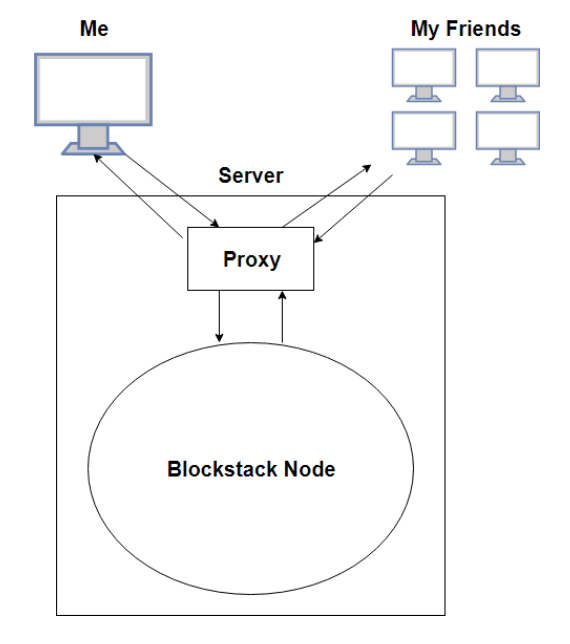
\includegraphics[scale=0.4]{pic1.jpg} \\
	\textbf{Figure 1}
\end{center}

In theory, the design of the system architecture of The Feed is supposed to provide the following properties:

\begin{center}
	\begin{itemize}
		\setlength{\itemsep}{2\baselineskip}
		\item A user can join the network at any time given that they have a .id namespace associated with Blockstack.
		\item A user has complete control over who is authorized to view/pull their data within the network
		\item At any time a user can completely remove their trace from the network without hindering the operation of the network.
	\end{itemize}
\end{center}

Below we present the design of each component and consider various tradeoffs.

\subsection{User Server}
\label{section:userserver}

The user-server is the most important component of The Feed as it dictactes how all operations take place on the network. Upon first signing into the The Feed a "user-server" is generated for the user. This is their private server which connects them to the network and handles all operations associated with participating in the network. The owner of a given user-server has full access (permissions) to all of the data stored on or through that user-server. All other users must first be granted access, by the owner, to the data reachable by that user-server. This is ensured through the authentication and permissions system described in section 3.3.\par
To connect the user to their storage and to the rest of the network, the user-server exposes an API which handles all requests. In version one of The Feed, the API performs the following functions:\newline

\begin{center}
	\begin{itemize}
		\setlength{\itemsep}{2\baselineskip}
		\item User Authorization and Permissions System
		\item Photo/Post Upload
		\item Photo/Post Retrieval
		\item Profile Retrieval/Updates
	\end{itemize}
\end{center}

\subsection{User Directory}
\label{section:userdirectory}

The user-directory is how The Feed provides connectivity i.e. how users can discover and follow each other within the network. This central node simply provides a mapping between a username and the IP address associated with that user's user-server. It supports related requests from a user such as:\newline	

\begin{center}
	\begin{itemize}
		\setlength{\itemsep}{2\baselineskip}
		\item Adding their user-server mapping to the directory
		\item Looking up another user in the network
		\item Removing their mapping from the directory\newline
	\end{itemize}
\end{center}	

	
The location of this user-directory is something that will be known to every user's user-server and therefore will be a "central" node. A possible drawback of this design decision is that a malicious entity could add a mapping to the directory claiming to own some Blockstack namespace. To combat this, the authorization and permissions system defined for the user-server will also be used to verify requests made to the user-directory.
	
\subsection{Authentication and Permissions}
\label{section:userauth}

Two things vital to the design of the The Feed are ensuring that users are indeed who they claim to be when making requests, and that a given user has permission to make said request. A two part authentication and verification systems is proposed that is standardized across every request is proposed as the following. A user must sign each request using the key tied to their Blockstack ID. Each request will be sent along with a user's Blockstack ID.\par
Upon receiving a request, the user's server will immediately authenticate and verify the sender by first setting a permission level for the request based on the user's Blockstack ID. If the user owns the server, then they are granted full access for the request. Otherwise access is granted on a per-request basis. To authenticate the requester, the server will retrieve the public key associated to the user's Blockstack ID and us this to verify the signed data. If the signature is valid, the server will then verify permissions to ensure that a non-owner is not trying to gain access to owner-only data. Once verified, the server will then decode the signed data and make sure that the request timestamp is within an appropriate range (for version 1 this is a few seconds). If a check fails at any point in this process, the server will respond with a failed result. Otherwise the server will send back the requested data.

\subsection{Storage}
\label{section:storage}

A graphical representation of the design of user storage is shown in \textbf{Figure 2}. The API design for user storage is presented below.\par

\begin{center}
	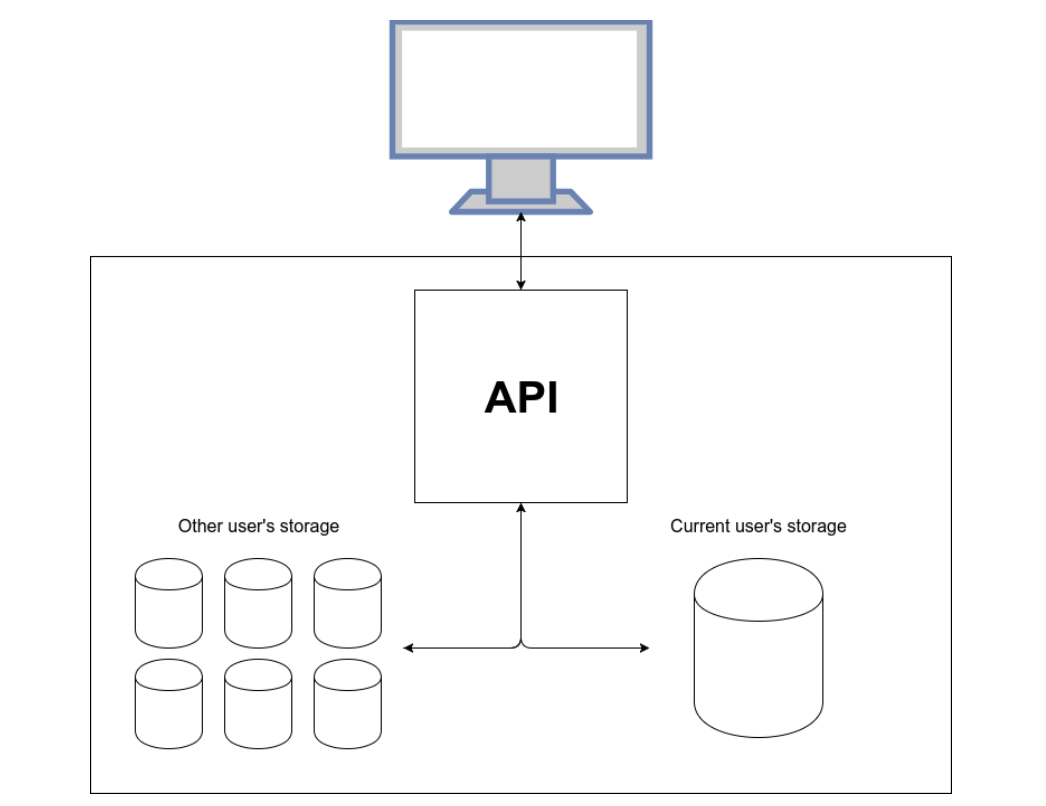
\includegraphics[scale=0.4]{pic3.jpg} \\
	\textbf{Figure 2}
\end{center}

The desired function of the storage is to give a user complete ownership their data on the network. A user should be able to define who has permission to view/pull their data from the network. Furthermore, at any point in operation a user should be able to \textbf{completely remove} all of their data from the network without hindering the operation of the rest of the network. To maintain these properties, each user provisions their own data storage (storage server) to pair with their user-server. As a result, for a user to pull data from every user that they follow their server must submit a separate request to each individuals user-server.\par
This performance tradeoff was made conciously to prevent a user's data from being stored and propagated throughout the network on the blockchain. This also completely eliminates the need for the expenditure of crypocurrency (transactions and associated fees) to register changes with the network. Furthermore, this slight degradation of performance is acceptable for a non-immediate form of content curation. If The Feed were, say, an instant messaging application this would be a critical design flaw.\newline

\subsection{Application}
\label{section:application}

A graphical representation of how the application interacts with the rest of the network is show in \textbf{Figrure 3}. The role of the application in the system architecture is described below.

\begin{center}
	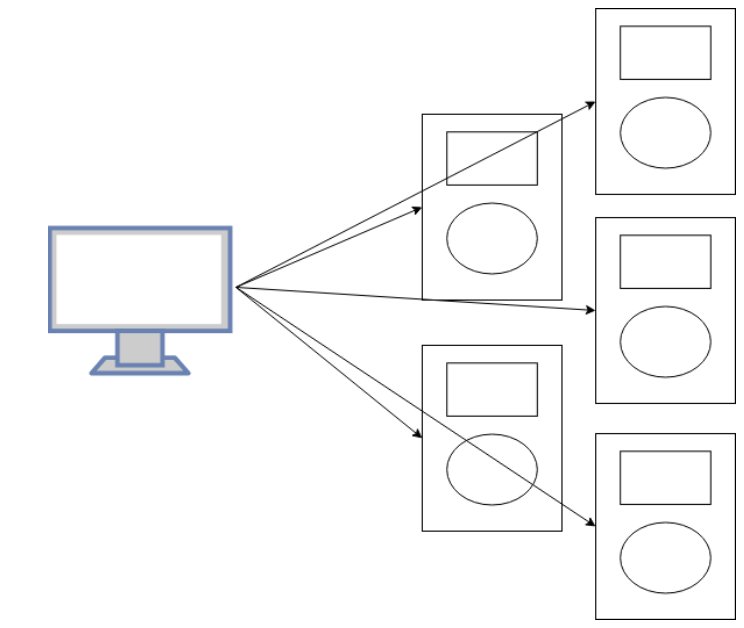
\includegraphics[scale=0.4]{pic2.jpg} \\
	\textbf{Figure 3}
\end{center}

The application runs locally in the user's browser. Essentially, the application provides the user with an interface through which they can access with the rest of the network. This serves web pages and forms requests for data that are submitted to a user-server. This design is the result of Blockstack having yet to release Multi-Reader Storage. Once this is released the system architecture will more resember \textbf{Figure 1}.

\subsection{Front End}
\label{section:frontend}

The front end directly handles how users interact with The Feed. Specifically, users can log in, view their profile page, view their feed,add followers, add photos, and add posts. The front end, beyond these set of features, must also populate a user's feed of posts and profile page because they will not be loaded automatically. This is especially important/tricky for viewing a user's feed and further discussion of how this is done in practice is presented in section 4.\newline

\section{Implementation}
\label{section:implementation}

Here a brief discussion of the implementation of The Feed is presented. The primary language for this project was javascript with use of the Node.js framework. Implementation consisted of setting up these three main components.

\subsection{User Server}
\label{section:server}

The user-server is implemented using the Node.js javascript framework (with express project generation) deployed to Google Cloud App Engine. The API exposed by the user-server are HTTP request handlers that implement all requests as POST requests so that the body of each request can be verified using the authentication and permission system.\par
The authorization and permissions system performs \quotes{signatures} through Javascript tokens which are encoded using the requester's Blockstack key. The Blockstack ID is submitted as argument along with the encoded data so that the user-server can retrieve the public key associated with the Blockstack ID to verify the signature and decode the token.\par 
The user storage is a simple MySQL (ClearDB) database deployed through the Heroku web service. Heroku allows independent database instances to be deployed and connected to from external web services. A user can configure their database instance directly from the command line.\par

\subsection{User Directory}
\label{section:directory}

The user-directory is very simple in implementation. This also a simple Node.JS deployed with Heroku (just like the user-servers storage) that handles HTTP requests through an exposed API. Upon initialization the database contains a single table which contains the mapping between.

\subsection{Application}
\label{section:app}

The application runs locally on the user's system. The user interacts with it through the browser. This is implemented using Node.js to create a local server and serve web content to the users browser. The application is also responsible for making signed and timestamped requests to the user's user-server and populating both the user's profile page and feed. Populating is a manual process for the user and can be done with the click of a button. On the application side, once the user requests for their profile page to be populated, the local server simply pulls the next posts waiting to be loaded. These are displayed in reverse time order. To populate a user's feed, their user-server will select 20 (or some other fixed number) of their followings randomly and request the next posts to be pulled from their servers.

\section{Benchmarks}
\label{section:benchmarks}

Although the above described implementation works, issues with the Blockstack service prevented us from collecting the performance data we had initially sought. Specifically, we wanted to measure how long it took, on average, for a user's feed to be loaded. Populating the feed, as described in the implementation section, presents a drag on the performance of the application as a request must be made to each individual user-server (maximum 20 per get-feed request) to pull data.\par
However, we were able to collect performance metrics on a few key operations related to the setup and participation in the network. Specifically, we have data collected on add-post requests (average of 20 requests). Most of the process involved with this request aplies to all others, thus we present the following:

\begin{center}
	(Times in ms)
	\begin{itemize}
		\setlength{\itemsep}{2\baselineskip}
		\item Average time to sign add-post request(browser side): 35.68
		\item Average public key retrieval time from Blockstack(server side): 109.50
		\item Average time to check a requester's signature(server side): 8.85
		\item Average time to insert post to database: 84.43
	\end{itemize}
\end{center}

Furthermore, \textbf{Figure 4} and \textbf{Figure 5} represent the effect of varying photo size on the add-post request and photo upload respectively.

\begin{center}
	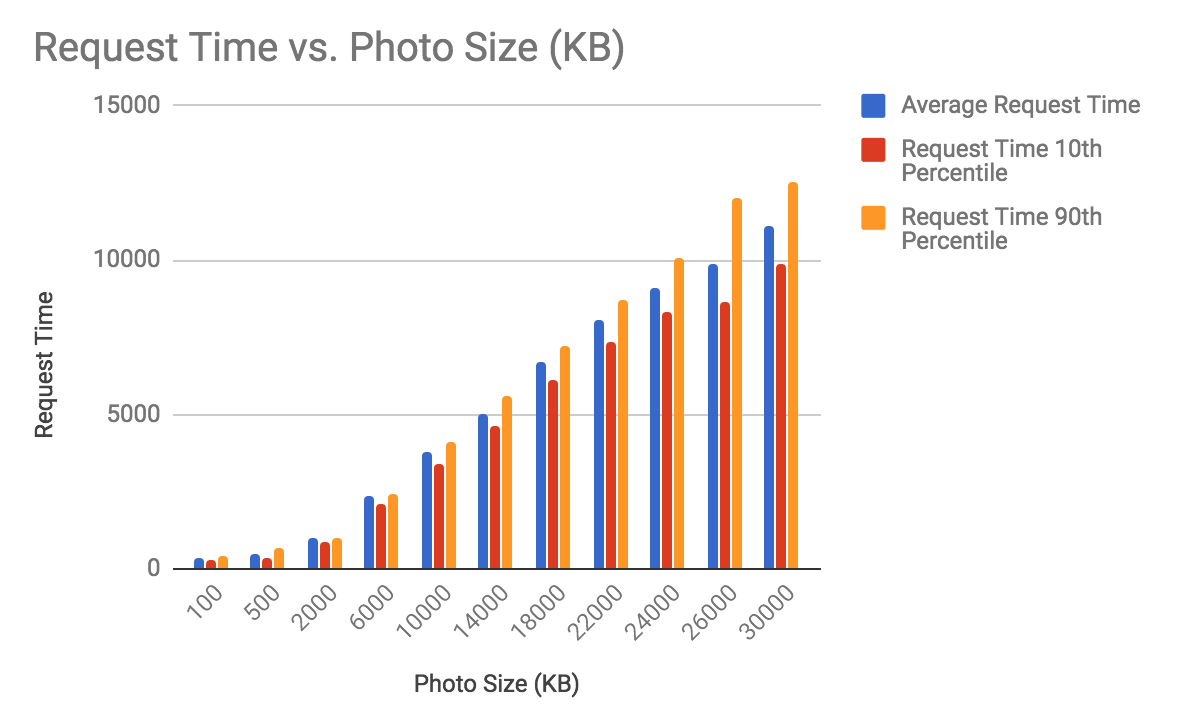
\includegraphics[scale=0.4]{request.jpg} \\
	\textbf{Figure 4}
\end{center}

\begin{center}
	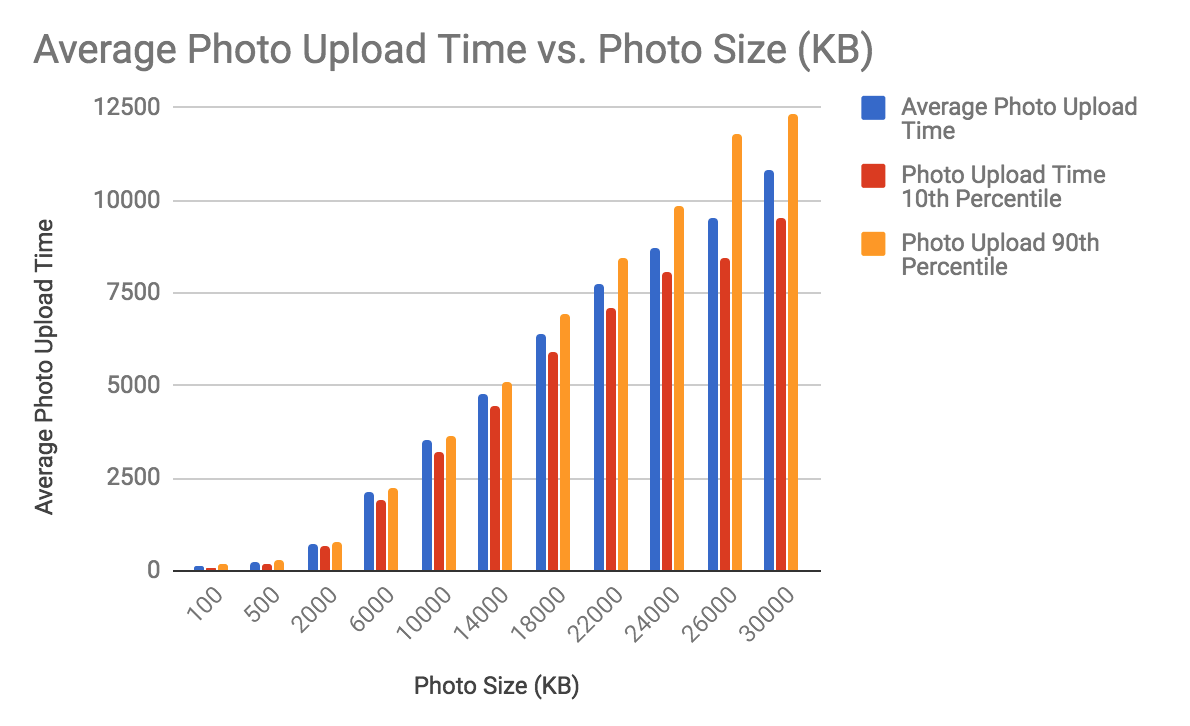
\includegraphics[scale=0.4]{photo.jpg} \\
	\textbf{Figure 5}
\end{center}

This data shows that our implementation of The Feed, even with the work around for Multi-Reader Storage, provides the user with adequate and consistent performance for key operations. 
\subsection{Bottlenecks and Limitations}
\label{section:bottlenecks}

When compared to traditional social networking applications (e.g Instagram), The Feed has several critical bottlenecks which hinder it's performance. First, note that setting up an account with a website like Instagram takes seconds not including email confirmation. The ease and speed with which a user can join the network is unparalleled in this regard as it takes several minutes, as noted above, to set up a single account with The Feed even with automation enabled.\par
The primary performance barrier is, as mentioned before, the population of a user's feed. In the current implementation at most 20 different user's are sent requests for populating the feed at a time. Another more serious limitation that stands out from this design is the cost of spinning up and running user-servers at scale. This hopefully won't be a problem in the future as Blockstack is currently working on releasing Multi-Reader Storage at the time of writing this paper.

\section{Conclusion}
\label{section:conclusion}

In this paper we introduce The Feed, a decentralize social networking application the provides users to completely own their data and do not have to trust a central "network overseer" with their content. The design of The Feed focuses on making reasonable performance tradeoffs to ensure that users within the network have as much control as possible over their data. Specifically, every user within the network runs the application locally, is provided with their own user-server, and controls access to their own user storage. For future work we plan to switch the system to Blockstack's Multi-Reader Storage once it is released. Version one of The Feed can be found on github at https://github.com/michaeljfriedman/IBOB. \newline


\bstctlcite{bstctl:etal, bstctl:nodash, bstctl:simpurl}
\bibliographystyle{IEEEtranS}
\bibliography{references}

\textit{I pledge my honor that I have not violated the University's regulations and that this paper represents my own work in accordance with the Princeton Honor Code.}\par
\end{multicols*}
\end{document}

